\documentclass[border=4pt]{standalone}
\usepackage[T1]{fontenc}
\usepackage[utf8]{inputenc}
\usepackage{lmodern}
\usepackage{tikz}
\usetikzlibrary{arrows.meta,calc}
\definecolor{azul}{HTML}{14334B}
\definecolor{acento}{HTML}{006699}
\definecolor{suave}{HTML}{EAF3F8}
\definecolor{ambar}{HTML}{94611C}
\begin{document}
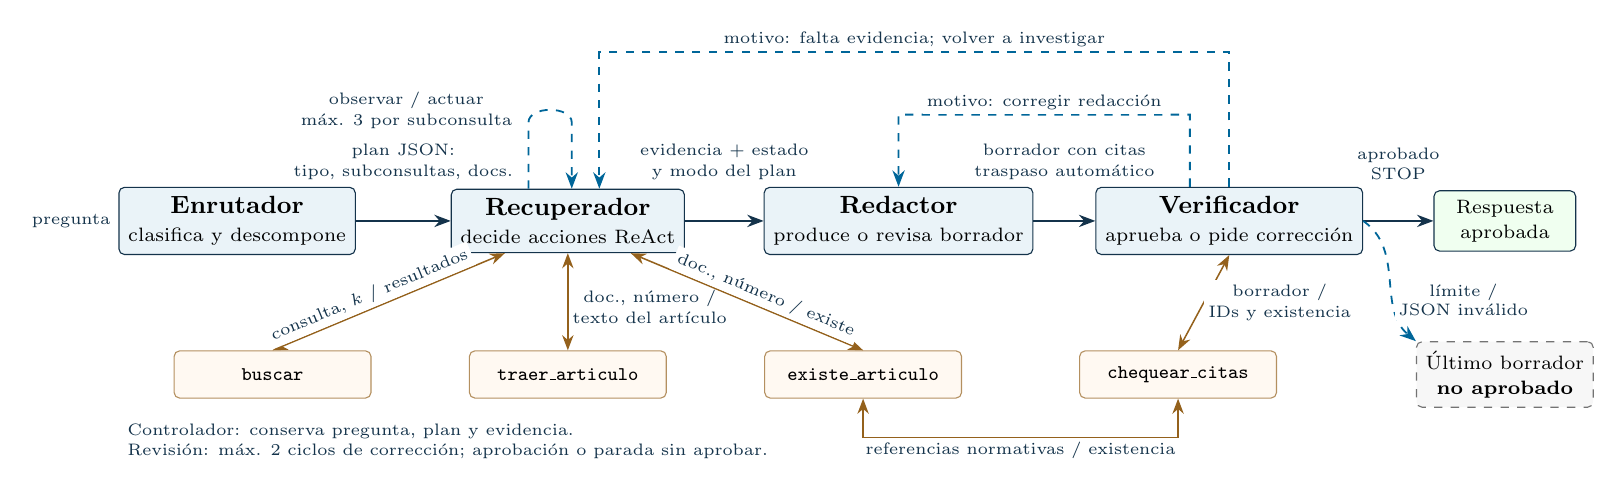
\begin{tikzpicture}[
 >=Stealth,
 agent/.style={draw=azul,fill=suave,rounded corners=2pt,minimum width=2.65cm,minimum height=0.78cm,align=center,font=\fontsize{9}{10}\selectfont},
 tool/.style={draw=ambar!70,fill=orange!5,rounded corners=2pt,minimum width=2.5cm,minimum height=0.6cm,align=center,font=\fontsize{7.5}{9}\selectfont},
 terminal/.style={draw=azul,fill=green!6,rounded corners=2pt,minimum width=1.8cm,minimum height=0.74cm,align=center,font=\fontsize{7.5}{9}\selectfont},
 lab/.style={fill=white,inner sep=1.5pt,align=center,font=\fontsize{6.5}{7.5}\selectfont,text=azul},
 flow/.style={->,draw=azul,line width=0.65pt},
 back/.style={->,draw=acento,dashed,line width=0.65pt},
 use/.style={<->,draw=ambar,line width=0.55pt}
]
\node[agent] (e) at (1.55,0) {\textbf{Enrutador}\\{\fontsize{7}{8}\selectfont clasifica y descompone}};
\node[agent] (r) at (5.75,0) {\textbf{Recuperador}\\{\fontsize{7}{8}\selectfont decide acciones ReAct}};
\node[agent] (w) at (9.95,0) {\textbf{Redactor}\\{\fontsize{7}{8}\selectfont produce o revisa borrador}};
\node[agent] (v) at (14.15,0) {\textbf{Verificador}\\{\fontsize{7}{8}\selectfont aprueba o pide corrección}};
\node[terminal] (out) at (17.65,0) {Respuesta\\aprobada};
\node[terminal,fill=black!3,draw=black!55,dashed] (stop) at (17.65,-1.95) {Último borrador\\\textbf{no aprobado}};

\draw[flow] (e.east)--node[lab,above=13pt]{plan JSON:\\tipo, subconsultas, docs.}(r.west);
\draw[flow] (r.east)--node[lab,above=13pt]{evidencia + estado\\y modo del plan}(w.west);
\draw[flow] (w.east)--node[lab,above=13pt]{borrador con citas\\traspaso automático}(v.west);
\draw[flow] (v.east)--node[lab,above=13pt]{aprobado\\STOP}(out.west);
\draw[back] (v.east) to[out=-35,in=140] node[lab,pos=.65,right,font=\fontsize{6}{7}\selectfont]{límite /\\JSON inválido}(stop.north west);
\node[lab,anchor=east] at (e.west) {pregunta\,};

\draw[back] ($(v.north)+(-.5,0)$) -- (13.65,1.35) -- node[lab,above,pos=.5]{motivo: corregir redacción} (9.95,1.35) -- (w.north);
\draw[back] (v.north) -- (14.15,2.15) -- node[lab,above]{motivo: falta evidencia; volver a investigar} (6.15,2.15) -- ($(r.north)+(.4,0)$);
\draw[back] ($(r.north)+(-.5,0)$) -- (5.25,1.25) to[out=90,in=90] (5.8,1.25) -- ($(r.north)+(.05,0)$);
\node[lab,anchor=east] at (5.1,1.4) {observar / actuar\\máx. 3 por subconsulta};

\node[tool] (b) at (2.0,-1.95) {\texttt{buscar}};
\node[tool] (a) at (5.75,-1.95) {\texttt{traer\_articulo}};
\node[tool] (x) at (9.5,-1.95) {\texttt{existe\_articulo}};
\node[tool] (c) at (13.5,-1.95) {\texttt{chequear\_citas}};
\draw[use] ($(r.south)+(-.8,0)$)--node[lab,pos=.56,sloped,above]{consulta, $k$ / resultados}(b.north);
\draw[use] (r.south)--node[lab,right,pos=.55]{doc., número /\\texto del artículo}(a.north);
\draw[use] ($(r.south)+(.8,0)$)--node[lab,pos=.56,sloped,above]{doc., número / existe}(x.north);
\draw[use] (v.south)--node[lab,right,pos=.5]{borrador /\\IDs y existencia}(c.north);
\draw[use] (c.south)--(13.5,-2.75)--node[lab,below]{referencias normativas / existencia}(9.5,-2.75)--(x.south);

\node[lab,anchor=west,align=left] at (0.1,-2.8) {Controlador: conserva pregunta, plan y evidencia.\\Revisión: máx. 2 ciclos de corrección; aprobación o parada sin aprobar.};
\end{tikzpicture}
\end{document}
